% Options for packages loaded elsewhere
\PassOptionsToPackage{unicode}{hyperref}
\PassOptionsToPackage{hyphens}{url}
\PassOptionsToPackage{dvipsnames,svgnames,x11names}{xcolor}
%
\documentclass[
  letterpaper,
  DIV=11,
  numbers=noendperiod,
  oneside]{scrartcl}

\usepackage{amsmath,amssymb}
\usepackage{iftex}
\ifPDFTeX
  \usepackage[T1]{fontenc}
  \usepackage[utf8]{inputenc}
  \usepackage{textcomp} % provide euro and other symbols
\else % if luatex or xetex
  \usepackage{unicode-math}
  \defaultfontfeatures{Scale=MatchLowercase}
  \defaultfontfeatures[\rmfamily]{Ligatures=TeX,Scale=1}
\fi
\usepackage{lmodern}
\ifPDFTeX\else  
    % xetex/luatex font selection
\fi
% Use upquote if available, for straight quotes in verbatim environments
\IfFileExists{upquote.sty}{\usepackage{upquote}}{}
\IfFileExists{microtype.sty}{% use microtype if available
  \usepackage[]{microtype}
  \UseMicrotypeSet[protrusion]{basicmath} % disable protrusion for tt fonts
}{}
\makeatletter
\@ifundefined{KOMAClassName}{% if non-KOMA class
  \IfFileExists{parskip.sty}{%
    \usepackage{parskip}
  }{% else
    \setlength{\parindent}{0pt}
    \setlength{\parskip}{6pt plus 2pt minus 1pt}}
}{% if KOMA class
  \KOMAoptions{parskip=half}}
\makeatother
\usepackage{xcolor}
\usepackage[left=1in,marginparwidth=2.0666666666667in,textwidth=4.1333333333333in,marginparsep=0.3in]{geometry}
\setlength{\emergencystretch}{3em} % prevent overfull lines
\setcounter{secnumdepth}{-\maxdimen} % remove section numbering
% Make \paragraph and \subparagraph free-standing
\makeatletter
\ifx\paragraph\undefined\else
  \let\oldparagraph\paragraph
  \renewcommand{\paragraph}{
    \@ifstar
      \xxxParagraphStar
      \xxxParagraphNoStar
  }
  \newcommand{\xxxParagraphStar}[1]{\oldparagraph*{#1}\mbox{}}
  \newcommand{\xxxParagraphNoStar}[1]{\oldparagraph{#1}\mbox{}}
\fi
\ifx\subparagraph\undefined\else
  \let\oldsubparagraph\subparagraph
  \renewcommand{\subparagraph}{
    \@ifstar
      \xxxSubParagraphStar
      \xxxSubParagraphNoStar
  }
  \newcommand{\xxxSubParagraphStar}[1]{\oldsubparagraph*{#1}\mbox{}}
  \newcommand{\xxxSubParagraphNoStar}[1]{\oldsubparagraph{#1}\mbox{}}
\fi
\makeatother

\usepackage{color}
\usepackage{fancyvrb}
\newcommand{\VerbBar}{|}
\newcommand{\VERB}{\Verb[commandchars=\\\{\}]}
\DefineVerbatimEnvironment{Highlighting}{Verbatim}{commandchars=\\\{\}}
% Add ',fontsize=\small' for more characters per line
\usepackage{framed}
\definecolor{shadecolor}{RGB}{241,243,245}
\newenvironment{Shaded}{\begin{snugshade}}{\end{snugshade}}
\newcommand{\AlertTok}[1]{\textcolor[rgb]{0.68,0.00,0.00}{#1}}
\newcommand{\AnnotationTok}[1]{\textcolor[rgb]{0.37,0.37,0.37}{#1}}
\newcommand{\AttributeTok}[1]{\textcolor[rgb]{0.40,0.45,0.13}{#1}}
\newcommand{\BaseNTok}[1]{\textcolor[rgb]{0.68,0.00,0.00}{#1}}
\newcommand{\BuiltInTok}[1]{\textcolor[rgb]{0.00,0.23,0.31}{#1}}
\newcommand{\CharTok}[1]{\textcolor[rgb]{0.13,0.47,0.30}{#1}}
\newcommand{\CommentTok}[1]{\textcolor[rgb]{0.37,0.37,0.37}{#1}}
\newcommand{\CommentVarTok}[1]{\textcolor[rgb]{0.37,0.37,0.37}{\textit{#1}}}
\newcommand{\ConstantTok}[1]{\textcolor[rgb]{0.56,0.35,0.01}{#1}}
\newcommand{\ControlFlowTok}[1]{\textcolor[rgb]{0.00,0.23,0.31}{\textbf{#1}}}
\newcommand{\DataTypeTok}[1]{\textcolor[rgb]{0.68,0.00,0.00}{#1}}
\newcommand{\DecValTok}[1]{\textcolor[rgb]{0.68,0.00,0.00}{#1}}
\newcommand{\DocumentationTok}[1]{\textcolor[rgb]{0.37,0.37,0.37}{\textit{#1}}}
\newcommand{\ErrorTok}[1]{\textcolor[rgb]{0.68,0.00,0.00}{#1}}
\newcommand{\ExtensionTok}[1]{\textcolor[rgb]{0.00,0.23,0.31}{#1}}
\newcommand{\FloatTok}[1]{\textcolor[rgb]{0.68,0.00,0.00}{#1}}
\newcommand{\FunctionTok}[1]{\textcolor[rgb]{0.28,0.35,0.67}{#1}}
\newcommand{\ImportTok}[1]{\textcolor[rgb]{0.00,0.46,0.62}{#1}}
\newcommand{\InformationTok}[1]{\textcolor[rgb]{0.37,0.37,0.37}{#1}}
\newcommand{\KeywordTok}[1]{\textcolor[rgb]{0.00,0.23,0.31}{\textbf{#1}}}
\newcommand{\NormalTok}[1]{\textcolor[rgb]{0.00,0.23,0.31}{#1}}
\newcommand{\OperatorTok}[1]{\textcolor[rgb]{0.37,0.37,0.37}{#1}}
\newcommand{\OtherTok}[1]{\textcolor[rgb]{0.00,0.23,0.31}{#1}}
\newcommand{\PreprocessorTok}[1]{\textcolor[rgb]{0.68,0.00,0.00}{#1}}
\newcommand{\RegionMarkerTok}[1]{\textcolor[rgb]{0.00,0.23,0.31}{#1}}
\newcommand{\SpecialCharTok}[1]{\textcolor[rgb]{0.37,0.37,0.37}{#1}}
\newcommand{\SpecialStringTok}[1]{\textcolor[rgb]{0.13,0.47,0.30}{#1}}
\newcommand{\StringTok}[1]{\textcolor[rgb]{0.13,0.47,0.30}{#1}}
\newcommand{\VariableTok}[1]{\textcolor[rgb]{0.07,0.07,0.07}{#1}}
\newcommand{\VerbatimStringTok}[1]{\textcolor[rgb]{0.13,0.47,0.30}{#1}}
\newcommand{\WarningTok}[1]{\textcolor[rgb]{0.37,0.37,0.37}{\textit{#1}}}

\providecommand{\tightlist}{%
  \setlength{\itemsep}{0pt}\setlength{\parskip}{0pt}}\usepackage{longtable,booktabs,array}
\usepackage{calc} % for calculating minipage widths
% Correct order of tables after \paragraph or \subparagraph
\usepackage{etoolbox}
\makeatletter
\patchcmd\longtable{\par}{\if@noskipsec\mbox{}\fi\par}{}{}
\makeatother
% Allow footnotes in longtable head/foot
\IfFileExists{footnotehyper.sty}{\usepackage{footnotehyper}}{\usepackage{footnote}}
\makesavenoteenv{longtable}
\usepackage{graphicx}
\makeatletter
\def\maxwidth{\ifdim\Gin@nat@width>\linewidth\linewidth\else\Gin@nat@width\fi}
\def\maxheight{\ifdim\Gin@nat@height>\textheight\textheight\else\Gin@nat@height\fi}
\makeatother
% Scale images if necessary, so that they will not overflow the page
% margins by default, and it is still possible to overwrite the defaults
% using explicit options in \includegraphics[width, height, ...]{}
\setkeys{Gin}{width=\maxwidth,height=\maxheight,keepaspectratio}
% Set default figure placement to htbp
\makeatletter
\def\fps@figure{htbp}
\makeatother

\KOMAoption{captions}{tableheading}
\makeatletter
\@ifpackageloaded{caption}{}{\usepackage{caption}}
\AtBeginDocument{%
\ifdefined\contentsname
  \renewcommand*\contentsname{Table of contents}
\else
  \newcommand\contentsname{Table of contents}
\fi
\ifdefined\listfigurename
  \renewcommand*\listfigurename{List of Figures}
\else
  \newcommand\listfigurename{List of Figures}
\fi
\ifdefined\listtablename
  \renewcommand*\listtablename{List of Tables}
\else
  \newcommand\listtablename{List of Tables}
\fi
\ifdefined\figurename
  \renewcommand*\figurename{Figure}
\else
  \newcommand\figurename{Figure}
\fi
\ifdefined\tablename
  \renewcommand*\tablename{Table}
\else
  \newcommand\tablename{Table}
\fi
}
\@ifpackageloaded{float}{}{\usepackage{float}}
\floatstyle{ruled}
\@ifundefined{c@chapter}{\newfloat{codelisting}{h}{lop}}{\newfloat{codelisting}{h}{lop}[chapter]}
\floatname{codelisting}{Listing}
\newcommand*\listoflistings{\listof{codelisting}{List of Listings}}
\makeatother
\makeatletter
\makeatother
\makeatletter
\@ifpackageloaded{caption}{}{\usepackage{caption}}
\@ifpackageloaded{subcaption}{}{\usepackage{subcaption}}
\makeatother
\makeatletter
\@ifpackageloaded{sidenotes}{}{\usepackage{sidenotes}}
\@ifpackageloaded{marginnote}{}{\usepackage{marginnote}}
\makeatother

\ifLuaTeX
  \usepackage{selnolig}  % disable illegal ligatures
\fi
\usepackage{bookmark}

\IfFileExists{xurl.sty}{\usepackage{xurl}}{} % add URL line breaks if available
\urlstyle{same} % disable monospaced font for URLs
\hypersetup{
  pdftitle={Ensembles Lab 2: Boosting},
  colorlinks=true,
  linkcolor={blue},
  filecolor={Maroon},
  citecolor={Blue},
  urlcolor={Blue},
  pdfcreator={LaTeX via pandoc}}


\title{Ensembles Lab 2: Boosting}
\author{Adapted by EVL, FRC and ASP}
\date{2025-03-07}

\begin{document}
\maketitle


\begin{Shaded}
\begin{Highlighting}[]
\CommentTok{\# Helper packages}
\FunctionTok{library}\NormalTok{(dplyr)       }\CommentTok{\# for data wrangling}
\FunctionTok{library}\NormalTok{(ggplot2)     }\CommentTok{\# for awesome plotting}
\FunctionTok{library}\NormalTok{(modeldata)  }
\FunctionTok{library}\NormalTok{(foreach)     }\CommentTok{\# for parallel processing with for loops}

\CommentTok{\# Modeling packages}
\CommentTok{\# library(tidymodels)}
\FunctionTok{library}\NormalTok{(xgboost)}
\FunctionTok{library}\NormalTok{(gbm)}
\end{Highlighting}
\end{Shaded}

\section{Introduction}\label{introduction}

This lab continues on the previous one showing how to apply boosting.
The same dataset as before will be used

\subsection{Ames Housing dataset}\label{ames-housing-dataset}

Packge \texttt{AmesHousing} contains the data jointly with some
instructions to create the required dataset.

We will use, however data from the \texttt{modeldata} package where some
preprocessing of the data has already been performed (see:
\url{https://www.tmwr.org/ames})

The dataset has 74 variables so a descriptive analysis is not provided.

\begin{Shaded}
\begin{Highlighting}[]
\FunctionTok{dim}\NormalTok{(ames)}
\end{Highlighting}
\end{Shaded}

\begin{verbatim}
[1] 2930   74
\end{verbatim}

\begin{Shaded}
\begin{Highlighting}[]
\FunctionTok{boxplot}\NormalTok{(ames)}
\end{Highlighting}
\end{Shaded}

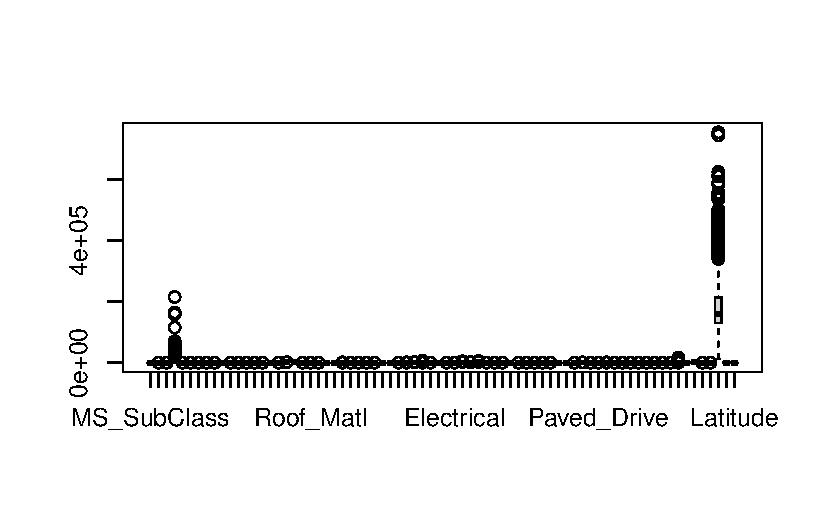
\includegraphics{Lab-C.2.4-Boosting_files/figure-pdf/unnamed-chunk-2-1.pdf}

We proceed as in the previous lab and divide the reponse variable by
1000 facilitate reviewing the results .

\begin{Shaded}
\begin{Highlighting}[]
\FunctionTok{require}\NormalTok{(dplyr)}
\NormalTok{ames }\OtherTok{\textless{}{-}}\NormalTok{ ames }\SpecialCharTok{\%\textgreater{}\%} \FunctionTok{mutate}\NormalTok{(}\AttributeTok{Sale\_Price =}\NormalTok{ Sale\_Price}\SpecialCharTok{/}\DecValTok{1000}\NormalTok{)}
\FunctionTok{boxplot}\NormalTok{(ames)}
\end{Highlighting}
\end{Shaded}

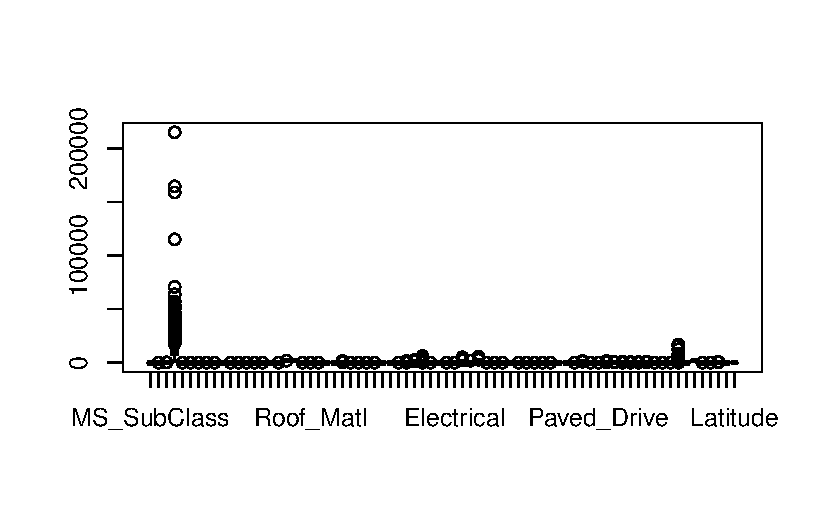
\includegraphics{Lab-C.2.4-Boosting_files/figure-pdf/unnamed-chunk-3-1.pdf}

\subsection{Spliting the data into
test/train}\label{spliting-the-data-into-testtrain}

The data are split in separate test / training sets and do it in such a
way that samplig is balanced for the response variable,
\texttt{Sale\_Price}.

\begin{Shaded}
\begin{Highlighting}[]
\CommentTok{\# Stratified sampling with the rsample package}
\FunctionTok{set.seed}\NormalTok{(}\DecValTok{123}\NormalTok{)}
\NormalTok{split }\OtherTok{\textless{}{-}}\NormalTok{ rsample}\SpecialCharTok{::}\FunctionTok{initial\_split}\NormalTok{(ames, }\AttributeTok{prop =} \FloatTok{0.7}\NormalTok{, }
                       \AttributeTok{strata =} \StringTok{"Sale\_Price"}\NormalTok{)}
\NormalTok{ames\_train  }\OtherTok{\textless{}{-}} \FunctionTok{training}\NormalTok{(split)}
\NormalTok{ames\_test   }\OtherTok{\textless{}{-}} \FunctionTok{testing}\NormalTok{(split)}
\end{Highlighting}
\end{Shaded}

\section{\texorpdfstring{Fitting a boosted regression tree with
\texttt{xgboost}}{Fitting a boosted regression tree with xgboost}}\label{fitting-a-boosted-regression-tree-with-xgboost}

\subsection{XGBoost Parameters
Overview}\label{xgboost-parameters-overview}

The \texttt{xgboost()} function in the XGBoost package trains Gradient
Boosting models for regression and classification tasks. Key parameters
and hyperparameters include:

\begin{itemize}
\tightlist
\item
  \textbf{Parameters}:

  \begin{itemize}
  \tightlist
  \item
    \texttt{params}: List of training parameters.
  \item
    \texttt{data}: Training data.
  \item
    \texttt{nrounds}: Number of boosting rounds.
  \item
    \texttt{watchlist}: Validation set for early stopping.
  \item
    \texttt{obj}: Custom objective function.
  \item
    \texttt{feval}: Custom evaluation function.
  \item
    \texttt{verbose}: Verbosity level.
  \item
    \texttt{print\_every\_n}: Print frequency.
  \item
    \texttt{early\_stopping\_rounds}: Rounds for early stopping.
  \item
    \texttt{maximize}: Maximize evaluation metric.
  \item
    \texttt{save\_period}: Model save frequency.
  \item
    \texttt{save\_name}: Name for saved model.
  \item
    \texttt{xgb\_model}: Existing XGBoost model.
  \item
    \texttt{callbacks}: List of callback functions.
  \end{itemize}
\end{itemize}

\subsubsection{XGBoost Parameters
Overview}\label{xgboost-parameters-overview-1}

Numerous parameters govern XGBoost's behavior. A detailed description of
all parameters can be found in the \texttt{XGBoost} documentation. Key
considerations include those controlling tree growth, model learning
rate, and early stopping to prevent overfitting:

\begin{itemize}
\tightlist
\item
  \textbf{Parameters}:

  \begin{itemize}
  \tightlist
  \item
    \texttt{booster} {[}default = gbtree{]}: Type of weak learner, trees
    (``gbtree'', ``dart'') or linear models (``gblinear'').
  \item
    \texttt{eta} {[}default=0.3, alias: learning\_rate{]}: Reduces each
    tree's contribution by multiplying its original influence by this
    value.
  \item
    \texttt{gamma} {[}default=0, alias: min\_split\_loss{]}: Minimum
    cost reduction required for a split to occur.
  \item
    \texttt{max\_depth} {[}default=6{]}: Maximum depth trees can reach.
  \item
    \texttt{subsample} {[}default=1{]}: Proportion of observations used
    for each tree's training. If less than 1, applies Stochastic
    Gradient Boosting.
  \item
    \texttt{colsample\_bytree}: Number of predictors considered at each
    split.
  \item
    \texttt{nrounds}: Number of boosting iterations, i.e., the number of
    models in the ensemble.
  \item
    \texttt{early\_stopping\_rounds}: Number of consecutive iterations
    without improvement to trigger early stopping. If NULL, early
    stopping is disabled. Requires a separate validation set (watchlist)
    for early stopping.
  \item
    \texttt{watchlist}: Validation set used for early stopping.
  \item
    \texttt{seed}: Seed for result reproducibility. Note: use
    \texttt{set.seed()} instead.
  \end{itemize}
\end{itemize}

\subsection{Test / Training in xGBoost}\label{test-training-in-xgboost}

\subsubsection{XGBoost Data Formats}\label{xgboost-data-formats}

XGBoost models can work with various data formats, including R matrices.

However, it's advisable to use \texttt{xgb.DMatrix}, a specialized and
optimized data structure within this library.

\begin{Shaded}
\begin{Highlighting}[]
\NormalTok{ames\_train }\OtherTok{\textless{}{-}} \FunctionTok{xgb.DMatrix}\NormalTok{(}
                \AttributeTok{data  =}\NormalTok{ ames\_train }\SpecialCharTok{\%\textgreater{}\%} \FunctionTok{select}\NormalTok{(}\SpecialCharTok{{-}}\NormalTok{Sale\_Price)}
                \SpecialCharTok{\%\textgreater{}\%} \FunctionTok{data.matrix}\NormalTok{(),}
                \AttributeTok{label =}\NormalTok{ ames\_train}\SpecialCharTok{$}\NormalTok{Sale\_Price,}
\NormalTok{               )}

\NormalTok{ames\_test }\OtherTok{\textless{}{-}} \FunctionTok{xgb.DMatrix}\NormalTok{(}
                \AttributeTok{data  =}\NormalTok{ ames\_test }\SpecialCharTok{\%\textgreater{}\%} \FunctionTok{select}\NormalTok{(}\SpecialCharTok{{-}}\NormalTok{Sale\_Price)}
                \SpecialCharTok{\%\textgreater{}\%} \FunctionTok{data.matrix}\NormalTok{(),}
                \AttributeTok{label =}\NormalTok{ ames\_test}\SpecialCharTok{$}\NormalTok{Sale\_Price}
\NormalTok{               )}
\end{Highlighting}
\end{Shaded}

\subsection{Fit the model}\label{fit-the-model}

\begin{Shaded}
\begin{Highlighting}[]
\FunctionTok{set.seed}\NormalTok{(}\DecValTok{123}\NormalTok{)}
\NormalTok{ames.boost }\OtherTok{\textless{}{-}} \FunctionTok{xgb.train}\NormalTok{(}
            \AttributeTok{data    =}\NormalTok{ ames\_train,}
            \AttributeTok{params  =} \FunctionTok{list}\NormalTok{(}\AttributeTok{max\_depth =} \DecValTok{2}\NormalTok{),}
            \AttributeTok{nrounds =} \DecValTok{1000}\NormalTok{,}
            \AttributeTok{eta=} \FloatTok{0.05}
\NormalTok{          )}
\NormalTok{ames.boost}
\end{Highlighting}
\end{Shaded}

\begin{verbatim}
##### xgb.Booster
raw: 872.5 Kb 
call:
  xgb.train(params = list(max_depth = 2), data = ames_train, nrounds = 1000, 
    eta = 0.05)
params (as set within xgb.train):
  max_depth = "2", eta = "0.05", validate_parameters = "1"
xgb.attributes:
  niter
callbacks:
  cb.print.evaluation(period = print_every_n)
# of features: 73 
niter: 1000
nfeatures : 73 
\end{verbatim}

\subsection{Prediction and model
assessment}\label{prediction-and-model-assessment}

\begin{Shaded}
\begin{Highlighting}[]
\NormalTok{ames.boost.trainpred }\OtherTok{\textless{}{-}} \FunctionTok{predict}\NormalTok{(ames.boost,}
                   \AttributeTok{newdata =}\NormalTok{ ames\_train}
\NormalTok{                 )}

\NormalTok{ames.boost.pred }\OtherTok{\textless{}{-}} \FunctionTok{predict}\NormalTok{(ames.boost,}
                   \AttributeTok{newdata =}\NormalTok{ ames\_test}
\NormalTok{                 )}

\NormalTok{train\_rmseboost }\OtherTok{\textless{}{-}} \FunctionTok{sqrt}\NormalTok{(}\FunctionTok{mean}\NormalTok{((ames.boost.trainpred }\SpecialCharTok{{-}} \FunctionTok{getinfo}\NormalTok{(ames\_train, }\StringTok{"label"}\NormalTok{))}\SpecialCharTok{\^{}}\DecValTok{2}\NormalTok{))}

\NormalTok{test\_rmseboost }\OtherTok{\textless{}{-}} \FunctionTok{sqrt}\NormalTok{(}\FunctionTok{mean}\NormalTok{((ames.boost.pred }\SpecialCharTok{{-}} \FunctionTok{getinfo}\NormalTok{(ames\_test, }\StringTok{"label"}\NormalTok{))}\SpecialCharTok{\^{}}\DecValTok{2}\NormalTok{))}

\FunctionTok{paste}\NormalTok{(}\StringTok{"Error train (rmse) in XGBoost:"}\NormalTok{, }\FunctionTok{round}\NormalTok{(train\_rmseboost,}\DecValTok{2}\NormalTok{))}
\end{Highlighting}
\end{Shaded}

\begin{verbatim}
[1] "Error train (rmse) in XGBoost: 14.31"
\end{verbatim}

\begin{Shaded}
\begin{Highlighting}[]
\FunctionTok{paste}\NormalTok{(}\StringTok{"Error test (rmse) in XGBoost:"}\NormalTok{, }\FunctionTok{round}\NormalTok{(test\_rmseboost,}\DecValTok{2}\NormalTok{))}
\end{Highlighting}
\end{Shaded}

\begin{verbatim}
[1] "Error test (rmse) in XGBoost: 22.69"
\end{verbatim}

\section{References}\label{references}




\end{document}
